

\subsection{1.21 Соединения переходных металлов 5 группы. Геометрия молекул в зависимости от природы лигандов, их электронное строение, способы получения и химическое поведение.}
\begin{itemize}
	\item $V$: $(+2), +3, +4, +5$ \quad $3d^34s^2$
	\item $Nb$: $(+2), (+3), (+4), +5$ \quad $4d^3 5s^2$
	\item $Ta$: $(+3), (+4), +5$ \quad $4f^{14} 5d^3 6s^2$
\end{itemize}
$V$:
\begin{itemize}
	\item $2(NH_4)_3VO_4 = t = V_2O_5 + 6 NH_3 + 3 H_2O$
	\item $V_2O_5 + 5 Ca = 5CaO + 2V$
\end{itemize}
$Ta, Nb$:
\begin{itemize}
	\item Вскрытие минералов, разделение
	\item Восстановление:
	\begin{align*}
		K_2(TaF_7) + 5 Na &= Ta + 2KF + 5 NaF \\
		Nb_2O_5 + 5C &= 2Nb + 5CO
	\end{align*}
\end{itemize}
Свойства:
\begin{itemize}
	\item $V$:
	\begin{itemize}
		\item $+ F_2 = VF_5$
		\item $+ KOH \not = $
		\item $+ O_2 = V_2O_5 $
		\item $+ HF = H_3\left[VF_6 \right] $
		\item $+ HNO_3(\text{к}) = VO_2NO_3 + NO_2 + H_2O$	
		\item $+ H_2SO_4 (\text{к}) = VO_SO_4 + SO_2 + H_2O  $
		\item $+ Br_2(I_2) = VBr_3(VI_3) $
		\item $+ Cl_2 = VCl_4 $	
	\end{itemize}
	\item $Nb, Ta$:
	\begin{itemize}
		\item $+ KOH \not = $
		\item $+ O_2 = Nb_2O_5 $
		\item $+ HF \not =  $
		\item $+ HNO_3(\text{к}) + HF = H_2\left[NbF_7 \right] + NO + H_2O $	
		\item $+ Cl_2 = NbCl_5 $		
	\end{itemize}
\end{itemize}
\textbf{Степень окисления $+2, +3$} ($d^3$) - основные свойства \\
$VaCl_3  + H_2 = VCl_2 + HCl$ \\
$NaVO_3 = Na/Hg, HCl = VCl_2 + NaCl + Hg + H_2O$ \\
Известны все $VHal_3$: $VF_3$ - н/р, остальные: $VCl_3 + H_2O = \left[V(H_2O)_6 \right]^{3+} + Cl^-  $ 
Восстановители:
\begin{align*}
VSO_4 + H_2SO_4 &= V_2(SO_4)_3 + H_2 \\	
VCl_3 + KMnO_4 + KOH &= KVO_3 + MnO_2 + KCl + H_2O 
\end{align*}
$V^{+3}, d^2$ - октаэдрические комплексы: $ \left[VCl_3(THF)_3 \right], \left[V_6 \right]^{3-}, \left[V(CO)_6 \right] $ \\
$V^{+2}, d^3$ - октаэдрические комплексы, в р-ре $ \left[V(H_2O)_6 \right]^{2+}, \left[V(CN)_6 \right]^{4-}, \left[V(phen)_3 \right]Cl_2 $ \\
\textbf{Степень окисления $+4$} - амфотерные свойства \\
$VO_2$ - структура рутила
\begin{align*}
NaVO_3 + N_2H_4 + H_2SO_4 &= VOSO_4 + N_2 + Na_2SO_4 + H_2O \\
V_2O_5 + H_2C_2O_4 &= t = VO_2 + CO_2 + H_2O
\end{align*}
Ванадильные комплексы:
\begin{figure} [H]
	\centering {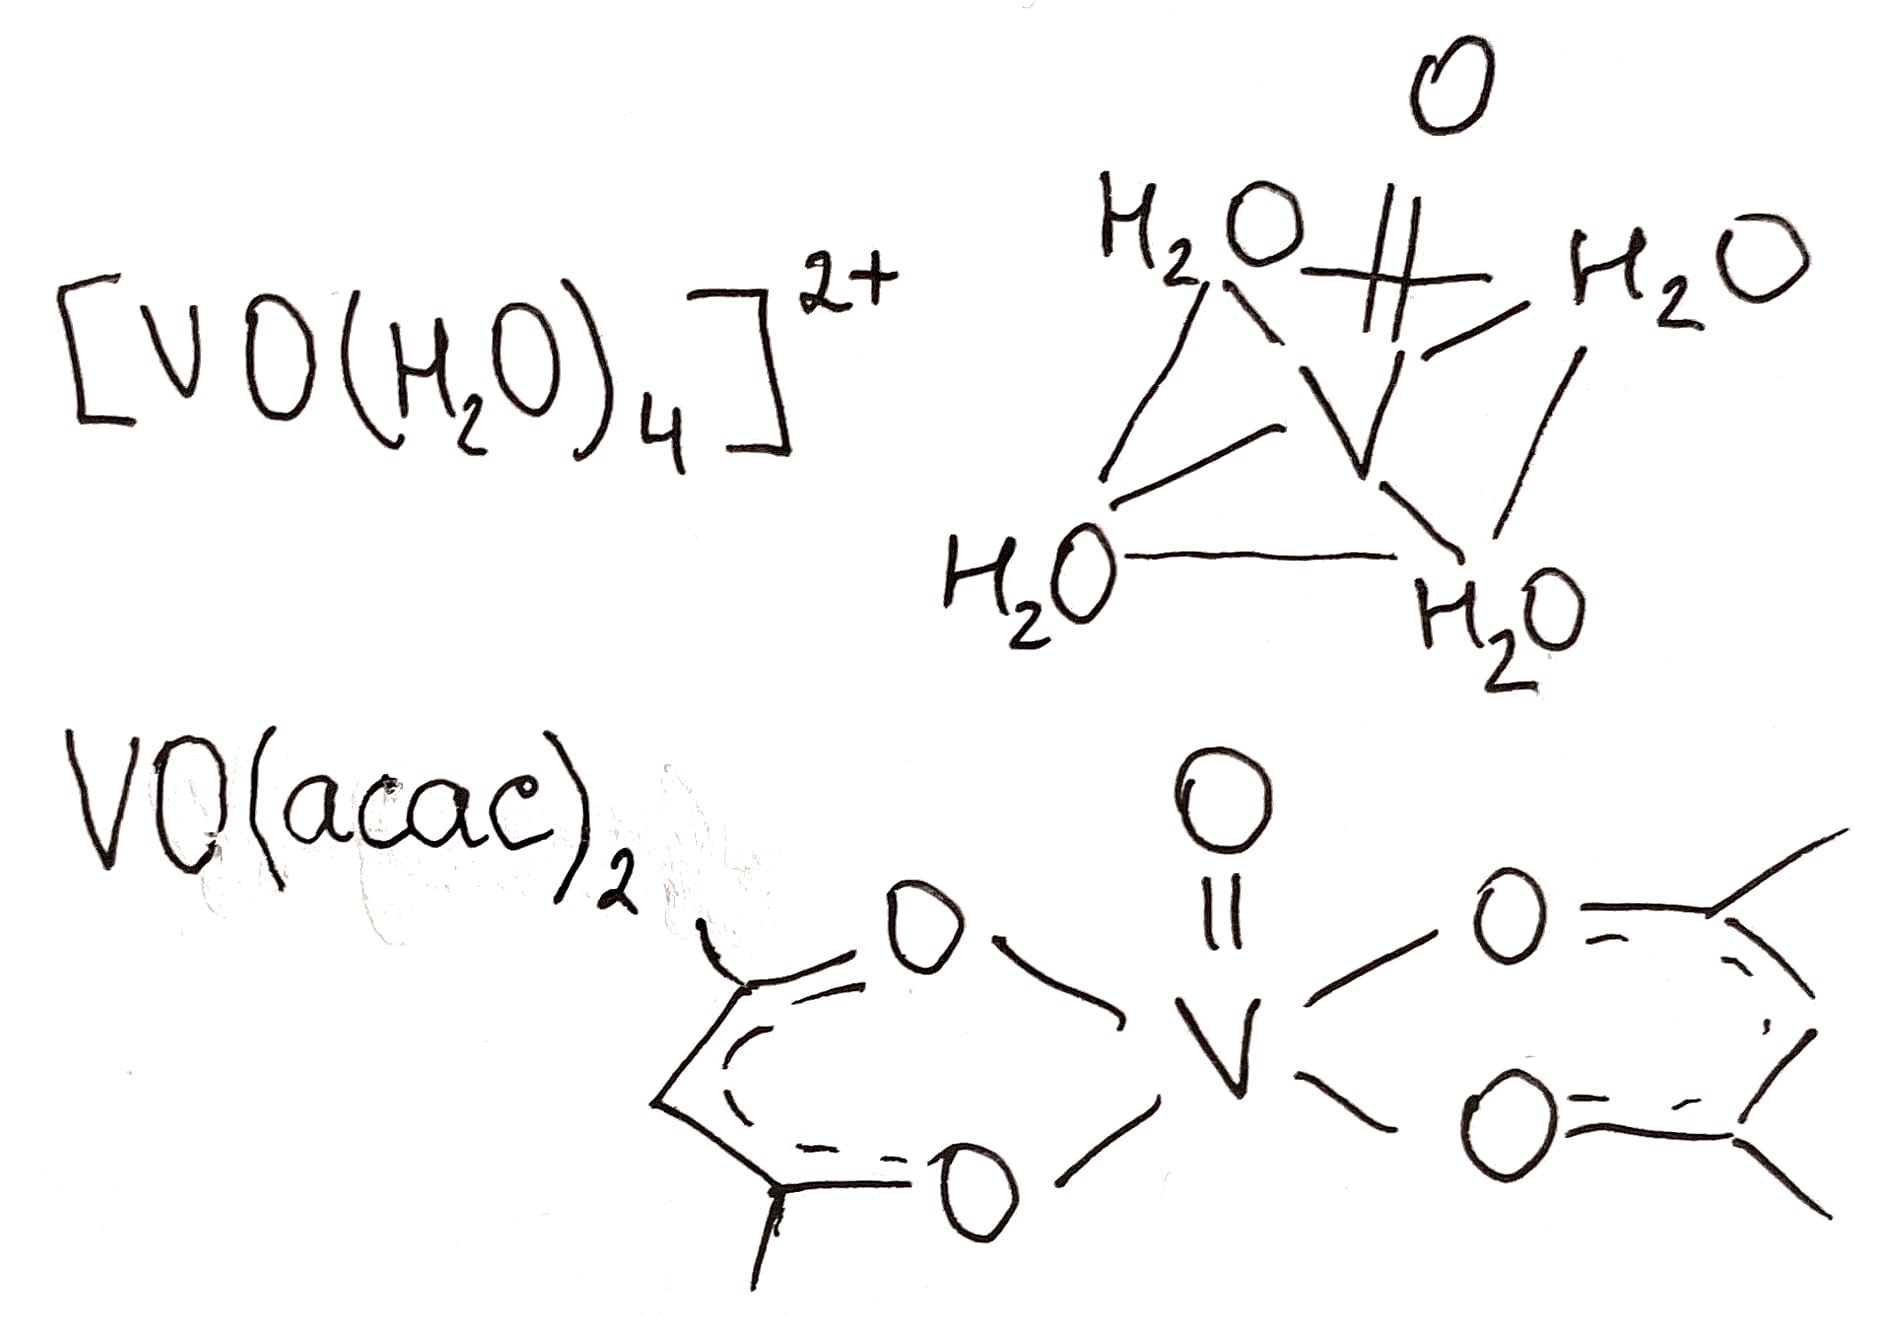
\includegraphics[scale=0.15]{ee1}}
\end{figure}
С $N-$донорными $L$: $(NH_4)_2\left[VOCl_4 \right]$ \\
$\left[VF_6 \right]^{2-}$ - октаэдр \\
$ 	\left[Nb(CN)_8 \right]^{4-}, \left[Nb(ox)_4 \right]^{4-} $ \\
\textbf{Степень окисления $+5$} - $V_2O_5$ - амфотерные свойства \\
В растворах $V^{+5}$ проявляет окислительные свойства \\
Гидролиз солей: $ NbCl_5 + H_2O = Nb_2O_5 \cdot H_2O + HCl $
Кислоты Льюиса: 
\begin{align*}
TaF_5 + BrF_3 &= \left[Br_2F_2 \right]\left[TaF_6 \right] \\
NbF_6 + KF &=   K_2\left[NbF_7 \right]
\end{align*}
$V^{+5}$ образует изо- и гетерополисоединения. \\
$VO_4^{3-}$ - тетраэдры \\
\[
\left[TaF_8 \right]^{3-} \quad \left[TaCl_5(bipy) \right] \quad \left[NbOCl_4 \right]
\] 
Фторидные комплексные анионы: $ \left[NbF_7 \right]^{2-}, \left[NbF_8 \right]^{3-} $ \\
В низших степенях окисления $Nb$ и $Ta$ образуют треугольные кластеры состава $M_3X_8$, октаэдрические кластеры $M_6X_{12}$

